\documentclass[a4paper]{report}
\usepackage[utf8x]{inputenc}
\usepackage[T1]{fontenc}
\usepackage[french]{babel}
\usepackage{graphicx}
\usepackage{fullpage}
\usepackage{eso-pic}
\usepackage{hyperref}
\usepackage{textcomp}
\usepackage{float}
\usepackage{appendix}
\usepackage{amsthm}
\usepackage{amsmath}
\usepackage{listings}
\usepackage{color}
\usepackage{subcaption}



\usepackage{array}

\definecolor{codegreen}{rgb}{0,0.6,0}
\definecolor{codegray}{rgb}{0.5,0.5,0.5}
\definecolor{codepurple}{rgb}{0.58,0,0.82}
\definecolor{backcolour}{rgb}{0.95,0.95,0.92}

\lstdefinestyle{mystyle}{
    backgroundcolor=\color{backcolour},
    commentstyle=\color{codegreen},
    keywordstyle=\color{magenta},
    numberstyle=\tiny\color{codegray},
    stringstyle=\color{codepurple},
    basicstyle=\ttfamily\footnotesize,
    breakatwhitespace=false,
    breaklines=true,
    captionpos=b,
    keepspaces=true,
    numbers=left,
    numbersep=5pt,
    showspaces=false,
    showstringspaces=false,
    showtabs=false,
    tabsize=2
}



\lstset{style=mystyle}
%\renewcommand{\thesection}{\arabic{section}}

%%\renewcommand\lstlistingname{Quelltext} % Change language of section name

%\providecommand{\tightlist}{%
%temsep}{0pt}\setlength{\parskip}{0pt}}

\providecommand{\tightlist}{}

\newcommand{\HRule}{\rule{\linewidth}{0.5mm}}
\newcommand{\blap}[1]{\vbox to 0pt{#1\vss}}
\newcommand\AtUpperLeftCorner[3]{%
  \put(\LenToUnit{#1},\LenToUnit{\dimexpr\paperheight-#2}){\blap{#3}}%
}
\newcommand\AtUpperRightCorner[3]{%
  \put(\LenToUnit{\dimexpr\paperwidth-#1},\LenToUnit{\dimexpr\paperheight-#2}){\blap{\llap{#3}}}%
}

\title{\LARGE{\begin{center}RAPPORT DE STAGE\end{center} \leavevmode\newline Classification des Cachalots par leurs clics}}
\author{\textsc{Arekion} Alexis\\M1 Informatique\\Année universitaire 2019/2020}
\date{\today}
\makeatletter

\begin{document}

\begin{titlepage}
    \enlargethispage{2cm}

    \AddToShipoutPicture{
        \AtUpperRightCorner{1.5cm}{1cm}{
\includegraphics[width=4cm]{./images/lamialogo.jpg}}
        \AtUpperLeftCorner{1cm}{0.5cm}{
\includegraphics[width=4cm]{./images/logoUA.jpg}}
    }
    \begin{center}
        \vspace*{1cm}
        
\includegraphics[width=6.5cm]{./images/Garde.jpg}
        \vspace*{0.5cm}

        \textsc{\@title}
        \HRule
        \vspace*{0.5cm}

        \large{\@author}
    \end{center}

    \begin{center}
      \vspace*{2cm}
      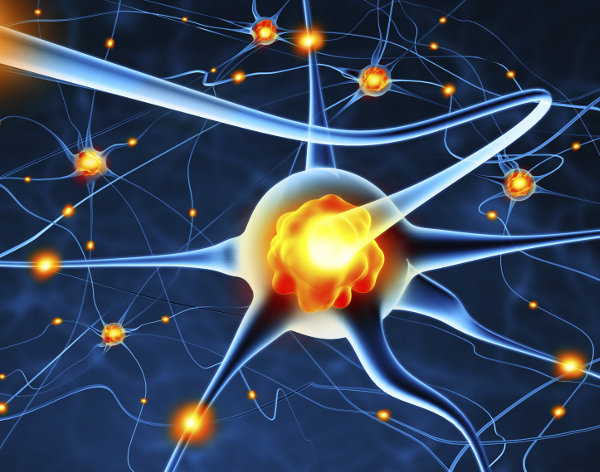
\includegraphics[width=6.5cm]{./images/n_a.jpg}
    \end{center}

    \vspace*{2cm}

    \begin{center}
        Université des Antilles

        Laboratoire de Mathématiques Informatique et Application (LAMIA)
        %\makebox[\textwidth]{
\includegraphics[width=\paperwidth]{./images/logoUA.jpg}}
    \end{center}

\end{titlepage}
\ClearShipoutPicture

\listoffigures
\tableofcontents

\hypertarget{Introduction}{%
\chapter{Introduction}\label{Introduction}}

\section{Présentation de la structure
d'accueil}

Durant la période de mon stage, j'ai été accueilli au sein du groupe \textbf{SpikeTrain} du 
\textbf{Laboratoire de Mathématiques Informatique et Applications
(LAMIA)} de l'\textbf{Université des Antilles (UA)}.
Je vais donc présenter ces trois entités, en commençant par l'Université des Antilles

\hypertarget{lUniversite-des-antilles}{%
\subsection{L'Université des Antilles}\label{luniversite-des-antilles}}

L'Université des Antilles est un public de l'enseignement supérieur qui entre dasn la catégorie des établissements à  caractère scientifique, culturel et professionnel (EPSCP).
Ces missions sont régies par l'article L123-3 du code de l'éducation :
\begin{itemize}
\item La formation initiale et continue tout au long de la vie ;
\item La recherche scientifique et technologique, la diffusion et la valorisation de ses résultats au service de la société ;
\item L’orientation, la promotion sociale et l’insertion professionnelle ;
\item La diffusion de la culture humaniste, en particulier à travers le développement des sciences humaines et sociales, et de la culture scientifique, technique et industrielle ;
\item La participation à la construction de l’Espace européen de l’enseignement supérieur et de la recherche ;
\item La coopération internationale.
\end{itemize} 

L'Université des Antilles s'organise autour deux pôles universitaires
régionaux dotés d'une certaine autonomie : le \textit{Pôle Guadeloupe} et le \textit{Pôle Martinique}.
Sur ces pôles, l'Université assure des missions de \emph{formation} et
de \emph{recherche}, par ses enseignants-chercheurs, Maîtres de Conférences ou Professeurs des Universités, ses chercheurs et ses enseignants, assistés par des personnels \emph{administratifs et 
techniques}.

\hypertarget{administration-et-personnel-technique}{%
\subsubsection{Administration et personnel
technique}
\label{administration-et-personnel-technique}}

l'UA emploie 414 agents administratifs et techniques (environ 200 personnes
pour l'administation centrale et 100 répartis sur chaque pôle)

\hypertarget{enseignements}{%
\subsubsection{Enseignements}\label{enseignements}}

L'UA délivre des diplomes de la licence au doctorat dans de nombreux
domaines. Au total, cela représente :

\begin{itemize}
\tightlist
\item
  484 enseignants-chercheurs (environ 240 pour chaque pôle)
\item
  12 000 étudiants (environ 7000 pour la Guadeloupe , 5000 pour la
  Martinique)
\end{itemize}

Pour l'informatique, cela représente : environ 20
enseignants-chercheurs pour 200 étudiants.

\hypertarget{recherche}{%
\subsubsection{Recherche}\label{recherche}}

La recherche à l'Université des Antilles est structurée en laboratoires auxquels sont rattachés les
enseignants chercheurs qui peuvent former de futurs chercheurs : les
doctorants.

L'Université compte ainsi au total :

\begin{itemize}
\tightlist
\item
  17 laboratoires
\item
  320 doctorants
\end{itemize}

Pour ma part, comme signalé précédemment, j'ai effectué mon stage dans
le laboratoire LAMIA que je vais maintenant présenter.

\hypertarget{le-lamia}{%
\subsection{Le laboratoire LAMIA}\label{le-lamia}}

Le \textbf{Laboratoire de Mathématiques Informatique et Application
(LAMIA)}, comme son nom l'indique, se concentre sur les recherches en
informatiques et mathématiques.

Il compte une soixantaine de membres (Professeurs des Universités,
Maitres de Conférences, ATER, Doctorants) répartis sur deux pôles
(Guadeloupe et Martinique) au sein de trois équipes internes :

\begin{itemize}
\tightlist
\item
  Equipe
  \href{http://lamia.univ-ag.fr/index.php?page=equipe-mathematiques}{\textbf{Mathématiques}
  (analyse variationnelle, analyse numérique, EDP, analyse statistique,
  mathématiques discrètes)} ;
\item
  Equipe Informatique
  \href{http://lamia.univ-ag.fr/index.php?page=equipe-danais}{\textbf{DANAIS}
  : Data analytics and big data gathering with sensors} ;
\item
  Equipe Informatique
  \href{http://lamia.univ-ag.fr/index.php?page=equipe-aid}{\textbf{AID}
  : Apprentissages Interactions Donnees} ;
\end{itemize}

De plus, le LAMIA accueille en son sein un groupe de chercheurs associés
travaillant en Epidémiologie clinique et médecine.

%L'équipe avec laquelle j'ai principalement travaillé est
%celle d'\textbf{Apprentissages Interactions Données} qui développe des
%méthodes de traitements et d'analyse de données hétérogènes : images
%(classique, multi-spectrale), séquences vidéos, séries temporelles et
%spatio-temporelles, dont la responsable est \textbf{Mme. Hélène
%Paugam-Moisy}.

Indépendamment de ces équipes, les travaux de recherche du laboratoire
se répartissent en \textbf{projets} qui peuvent réunir des membres de
plusieurs équipes en \textbf{groupes de travail}. Mon stage était en
fait plus attaché à un projet et un groupe de travail qu'à une équipe.

Ce groupe de travail, nommé SpikeTrain,  et
concerne l'utilisation de \textbf{réseaux de neurones impulsionnels}
pour l'apprentissage automatique (ces notions seront définies plus
loin). Le groupe de travail associé réunit à l'heure actuelle :

\begin{itemize}
\tightlist
\item
  1 Professeur des Universités
\item
  2 MCF avec HDR
\item
  3 MCF
\item
  1 ingénieur d'études.
\end{itemize}.

C'est avec ces personnes que j'ai travaillé tout au long du stage et mes
tuteurs de stage était \textbf{M.~Vincent PAGÉ et M. ~Manuel CLERGUE}.

%Ci dessous, un schéma présentant la structure du laboratoire me
%rattachant à cette structure. (L'équipe de travail \textbf{Spikestrain}
%étant informelle, elle ne figure pas sur ce schéma.)
%
%\begin{figure}[h!]
%\centering
%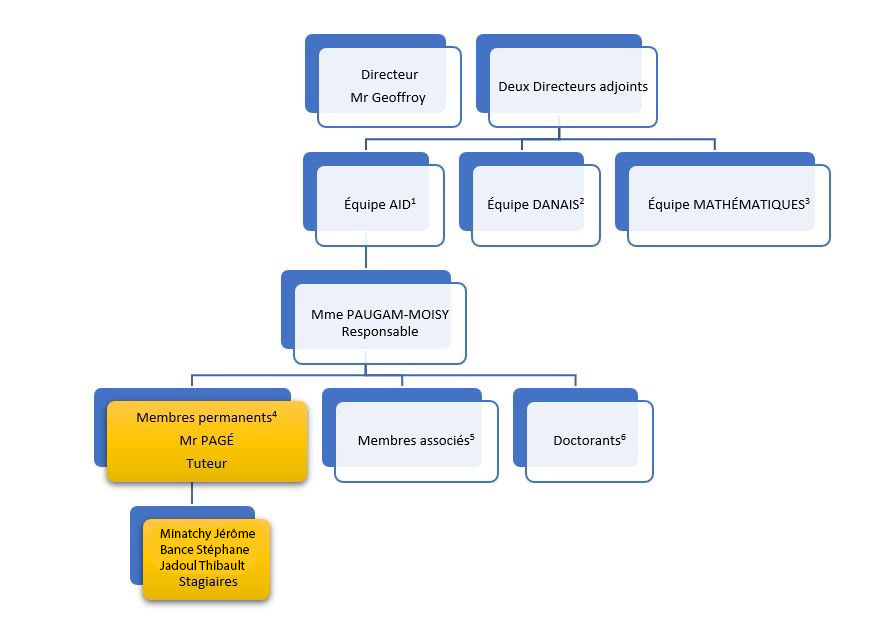
\includegraphics[width=10cm]{./images/orga.jpg}
%\caption{Figure 1 Schéma de l'organisation interne du LAMIA:
%¹Apprentissages Interactions Données. ²Data analytics and big data
%gathering with sensors. ³Mathématiques (analyse variationnelle, analyse
%numérique, EDP, analyse statistique, mathématiques discrètes). ⁴Membres
%permanents : Suzy Gaucher-Casalis~(MCF),~Enguerran
%Grandchamp~(MCF--HDR),~Jean-Luc Henry~(MCF),~Jimmy Nagau~(MCF),~Vincent
%Pagé(MCF),~Helene Paugam Moisy~(PR),~Sébastien Régis~(MCF),~Céline
%Rémi~(MCF).}
%\end{figure}

La prochaine section sera consacrée à la présentation de la thématique
de recherche du groupe SpikesTrain et de mon stage.


\hypertarget{Objectif_Spike}{%
\subsection{Le groupe Spiketrain}\label{Groupe_Spiketrain}}

Le groupe \textbf{Spikestrain} s'intéresse aux techniques
d'\textbf{Intelligence Artificielle}, plus spécifiquement à
l'\textbf{apprentissage automatique} dont l'objectif est de créer des
programmes capable d'apprendre à partir de bases d'exemples.

Actuellement, parmi les techniques permettant l'apprentissage
automatique, une se démarque et est très populaire : les
\textbf{réseaux de neurones artificiels}, notamment dans leur version
\emph{profonde} qui sont très utilisés par exemple par \textbf{Facebook™}
pour sa \textbf{reconnaissance faciale} ou encore par \textbf{Google™}
pour ses \textbf{robots} qui apprennent par \textbf{répétitions} à jouer
à des jeux de stratégies comme les échecs ou le Go.


\hypertarget{Contexte}{%
\section{Contexte du stage}\label{Contexte}}

\hypertarget{Le-Challenge}{%
\subsection{Le Challenge: Classifier les Cachalots}\label{Le-Challenge}}

Le challenge "Dyni Odontocete Click Classification" (https://challengedata.ens.fr/challenges/32) consiste à réaliser un classifieur qui classe des mammifères marins de dix espèces différentes à partir de leurs "clics", c'est à dire le son qu'ils émettent avec leur machoires.
Pour celà nous avions à disposition une base d'apprentissage labelisée (comportant 113000 exemples) ainsi qu'une base de test non labelisée (comportant 20000 exemples) sur laquelle nous pouvions évaluer les performances réelles de nos classifieurs. 
%Pour cela nous labelision les exemples de la base non labelisée puis nous envoyions nos prédictions sur le site du challenge qui nous renvoyais nos performances ainsi qu'un classement des performances de tous les participants.

Les deux bases sont constituées d'enregistrements audios des clics des différentes espèces. Chaque enregistrement contient 8192 mesures faites à une fréquence d'échantillonnage de 200KHz. Dans le cas de la base non labelisée appellée base de test chaque enregistrement contient normalement un clic centré au milieu de la fenêtre tandis que dans la base labelisée appellée base d'apprentissage, le clic n'est pas spécialement centré et peut se situer à divers moments de l'enregistrement. De plus, les enregistrements peuvent contenir divers bruits.

L'objectif est de classer chaque enregistrement en fonction de l'espèce émettrice correspondante. Les 10 espèces sont : 
\begin{itemize}
\item (0) Gg : Grampus griseus- Dauphin de Risso 
\item (1) Gma : Globicephala macrorhynchus- Baleine pilote à nageoires courtes 
\item (2) La : Lagenorhynchus acutus- Dauphin à flancs blancs de l'Atlantique 
\item (3) Mb : Mesoplodon bidens- Baleine à bec de Sowerby 
\item (4) Me : Mesoplodon europaeus- Baleine à bec de Gervais 
\item (5) Pm : Physeter macrocephalus - Cachalot 
\item (6) Ssp : Stenella sp.Dauphin stenellide 
\item (7) UDA : Delphinidés de type A - un groupe de dauphins (espèces non encore déterminées)
\item (8) UDB : Delphinidés de type B - un autre groupe de dauphins (espèces non encore déterminées) 
\item (9) Zc : Ziphius cavirostris - Baleine de Cuvier à bec.
\end{itemize}

La performance du classifieur est évaluée sur la base de test (les labels sont envoyés au site du challenge) par une mesure d'accuracy (le nombre de bien classés sur le nombre total d'exemples).

\hypertarget{Etat-des-lieux-lors-de-mon-arrivuxe9}{%
\subsection{Etat des lieux à mon arrivé}
\label{Etat-des-lieux-lors-de-mon-arrivuxe9}}

Quand j'ai commencé mon stage, mes tuteurs avaient déjà commencé le challenge depuis un moment déjà c'est pourquoi j'ai dû dans un premier temps me mettre à jour sur le challenge et ce qu'ils avaient fait, à savoir :
\begin{itemize}
\item Un grand nombre de tentatives de résolution du probléme uniquement basé sur du machine learning notament des réseaux de neurones et des réseaux de neurones convolutifs
\item Divers traitements des signaux bruts
\item De l'augmentation de données
\end{itemize}



Leurs meilleurs résultats étaient de l'ordre de 98\% de réussite en accuracy sur la base labelisée contre 72 \% de réussite sur la base non labelisée, soit un écart de 20 pourcents de réussite entre les deux bases qui persistait même en utilisant d'autres méthodes de machine learning donnant de moins bons résultats.
Cet important différentiel est d'autant plus surprenant que les auteurs du challenge nous présentent les données de la base non labelisée comme des données de meilleure qualité que celles de la base labelisée.

C'est pour mieux comprendre ce différentiel mais surtout le probléme dans son ensemble que j'ai été chargé de créer un certain nombre d'outils facilitant l'analyse et la visualisation des données et des effets des traitements que nous leurs appliquons.

Mais avant de pouvoir commencer cette partie du travail il a fallu commencer par comprendre un certaine nombre d'outils et de concepts que nous allons voir ensemble.


\hypertarget{Neurone-artificiel}{%
\subsubsection{Neurone artificiel}
\label{Neurone-artificiel}}
Tout d'abord avant de parler de réseaux de neurones il faut expliquer le principe du neurone artificiel.

Un neurone artificiel est pourvu d'un certain nombre d'\textbf{entrées}. Dans le cas des neurones classiques, ces entrées sont des nombres réels. Le neurone calculera, en fonction de ces entrées, une unique valeur en \textbf{sortie}.
Détaillons la façon dont ces calculs sont effectués:

Chacune de ces entrées circule sur une connection, laquelle est caractérisée par un \textbf{poids} qui définit l'importance de l'entrée pour le neurone.

Le neurone calcule dans un premier temps la somme de ses entrées, pondérée par leurs poids respectifs, à laquel vient s'ajouter un \textbf{biais} spécifique à chaque neurone (cf. equation~\ref{sommePonderee}).

\begin{equation}
\label{sommePonderee}
y = \sum_{i}^{n} w_i \times x_i + b
\end{equation}

Le résultat de cette somme passe alors dans une \textbf{fonction d'activation} qui permet d'introduire une non-linéarité dans les calculs. La sortie $s$ du neurone est donc calculée conformément à l'équation~\ref{calcNeurone}

\begin{equation}
\label{calcNeurone}
s = f(\sum_{s=0}^{n_{x}} x_{n}w_{n} + b)
\end{equation}

Un schéma reprenant ces explications est présenté dans la figure~\ref{neuroneSeul}.

\begin{figure}[h]
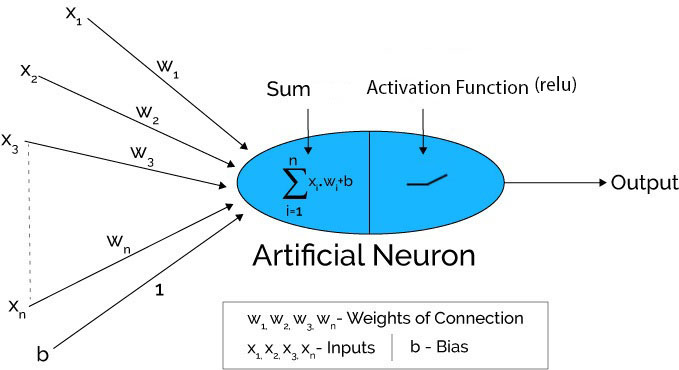
\includegraphics[width=16.5cm]{./images/image2.jpg}
\caption{Fonctionnement d'un neurone seul.\label{neuroneSeul}}
\end{figure}

Notre apprentissage se fera en modifiant les poids de ses différentes
connexions (et le biais) de façon à obtenir une sortie proche de celle voulu.\newline

\hypertarget{Ruxe9seau-de-neurones-classique}{%
\subsection{Réseau de neurones classique}
\label{Ruxe9seau-de-neurones-classique}}

Les neurones présentés précédemment prennent tout leur intérêt lorsqu'ils sont utilisés en groupes, dans des \textbf{réseaux de neurones}.

Le premier de ces réseaux, encore utilisé de nos jours, est appelé \textbf{perceptron}.
Le principe du perceptron n'est pas nouveau et date des années 1960.

Dans ces types de réseaux, les neurones sont organisés en \textbf{couches} (une seul couche pour le perceptron et plusieurs pour le perceptron multicouche).
La première couche correspond à celle qui permettra d'introduire des informations dans le réseau (comme la rétine par exemple). Elle est nommée \textbf{couche d'entrée}
La dernière couche permettra de lire les décisions du réseau. Elle est appelée \textbf{couche de sortie}. Dans les applications classiques, à chaque neurone de la couche de sortie correspond une décision possible et le neurone qui est le plus activé sur la couche de sortie l'emporte.
Entre ces couches, on trouve souvent un nombre variable de couches intermédiaires appelées \textbf{couches cachées}.

Entre deux couches, on établit le plus souvent un schéma de connexion que nous pouvons qualifier de \textit{full connected}, c'est à dire que chaque neurone d'une couche est connecté avec chaque neurone de la couche suivante.Nous allons encore une fois, pour le bien de ce rapport, ne pas épiloguer sur les autres types de connexions existantes.\newline

Ce type d'architecture est présentée sur la figure \ref{reseauClassique}.

\begin{figure}[h]
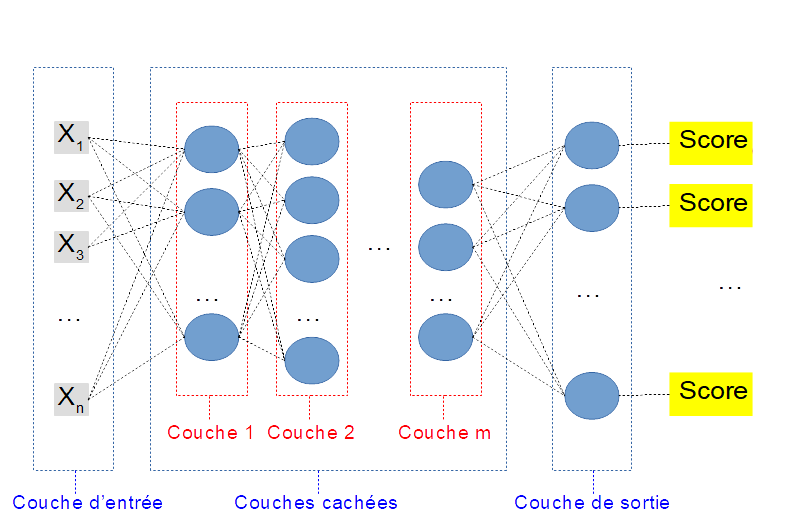
\includegraphics[width=16.5cm]{./images/multicouche.png}
\caption{réseau de neurones classique en couches.%
\label{reseauClassique}}
\end{figure}


\hypertarget{Ruxe9seau-de-neurones-convolutif}{%
\subsection{Réseau de neurones convolutifs}
\label{Ruxe9seau-de-neurones-convolutif}}

le réseau de neurones convolutifs est un type de réseau de neurones
inspiré par le cortex cérébral des animaux.
Il possède de larges applications dans la reconnaissance d'images, de vidéos et de sons.

Ce réseau se présente comme un réseau classique , une couche d'entrée,
une couche de sortie et des couches cachées.
Ces couches cachées possèdent des couches \textbf{convolutives}
pour lesquelles chaque neurone va appliquer un filtre convolutif
sur une partie de l'image en entrée afin d'analyser toute l'image
(voir figure \ref{fig:explication_convolution}).

\begin{figure}[h!]
\begin{center}
\centering
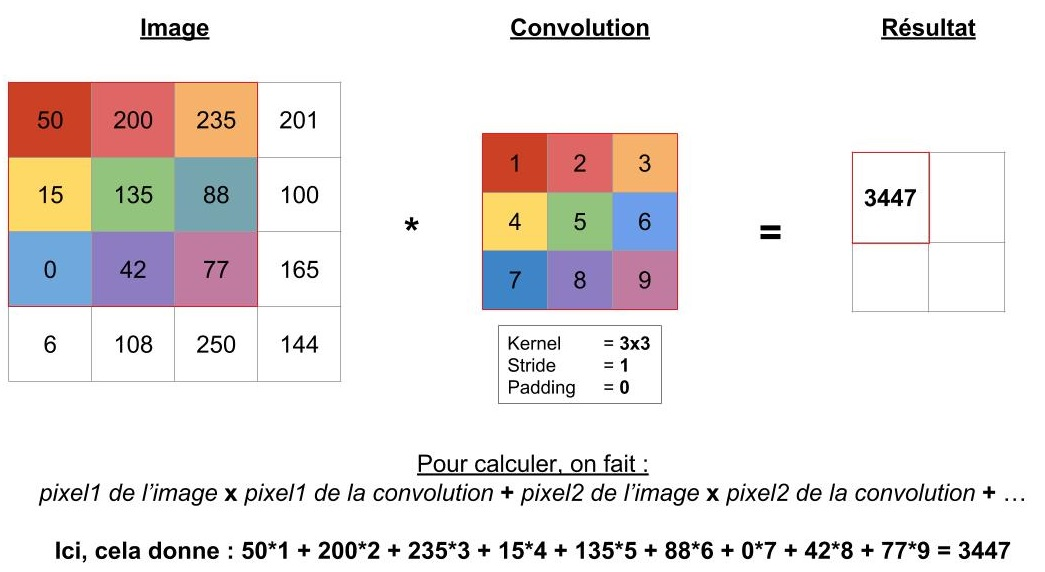
\includegraphics[width=15cm]{./images/explication_convolution.jpg}
\caption[Schéma de la convolution.]{L'image d'entrée est découpée en \textit{patchs}
sur lesquels est appliqué un filtre de convolution.
La sortie de ce fitre appliqué à chacun des patchs donne la couche de sortie
de la couche convolutive (appelée carte ou map).
La convolution est paramètrée par : le \textit{kernel} (la forme du patch),
le \textit{stride} (le déplacement du filtre) et le \textit{padding}
 (la façon dont les bords de l'image vont être traités).\label{fig:explication_convolution}}
\end{center}
\end{figure}

Ces neurones ont souvent une fonction d'activation de type \textit{Relu}
qui borne l'activation du neurone à 0. Ce sont donc des neurones
dont l'activation ne peut être que positive ou nulle.

Les réseaux convolutifs possèdent aussi des couches de \textbf{pooling}.
Le \textbf{pooling} est une opération simple qui consiste à remplacer une zone de pixels
(généralement 2×2 ou 3×3) par une valeur unique (généralement le max ou la moyenne).
De cette manière, l’image diminue en taille et se retrouve simplifiée (lissée).

L'un des intérêts majeurs des réseaux convolutifs est qu'ils permettent de réaliser une invariance
de translation : un motif appris sur une zone de l'image sera reconnue
quelque soit sa position dans l'image.
Un autre intérêt est qu'ils nécessitent l'apprentissage de beaucoup moins de paramètres (les poids) que les réseaux de neurones de type Perceptron Multicouche, pour des performances 
en classification équivalentes ou supérieures.

\hypertarget{Tensorflow}{%
\subsection{TensorFlow}%
\label{Tensorflow}}

\comment{à renvoyer vers la section outils}

\begin{center}
\label{fig:Tensorflow_logo}
\centering

\includegraphics[width=5cm]{./images/Tensorflow_logo.png}
\begin{figure}[h!]
\caption{Logo de Tensorflow}
\end{figure}
\end{center}


TensorFlow est un framework open source,
multiplateforme d'apprentissage automatique développée par Google Brain,
en C++ avec une interface pour Python.
Sa premiere version est publiée par Google le 9 novembre 2015.
L'intérêt de ce framework est de limiter les coûts de développement des solutions à base
de réseaux de neurones, en réunissant des fonctionnalités permettant,
en quelques lignes de code de construire des réseaux complexes.
Tensorflow permet donc de simplifier beaucoup de choses dans
le domaine de l'apprentissage automatique.
Son autre intérêt est de fournir des interfaces pour pouvoir exécuter les calculs sur
des accélérateurs graphiques et surtout de les prendre en charge
de façon complétement transparente pour les utilisateurs.
Les gains de vitesse peuvent atteindre ainsi un facteur 10 quand le même modèle est exécuté
sur une carte graphique.

Le concurrent principal de TensorFlow est pyTorch, utilisé par FaceBook.

\hypertarget{plan}{%
\section{Présentation du plan du rapport}%
\label{Présentation du plan du rapport}}


\hypertarget{Analyse-et-traitement-des-donnuxe9es}
\section{Les signaux}
\label{Les-signaux}}

Afin d'améliorer la lisibilité des chapitres suivants nous prendrons 3 signaux (le n°17000 et le n°20000 de la base labelisée ainsi que le n°571 de la base non labelisée) que nous observerons sous diverses formes puis sur lesquels nous effectuerons un certain nombre de traitements.

\hypertarget{Signaux-Bruts}{%}
\subsection{Signaux Bruts}
\label{Signaux-Bruts}}

Dans un premier temps on commence par observer les signaux sans traitement sous différentes formes.\n
D'abord de manière brute :

\begin{figure}[!h]
  \centering
  \begin{subfigure}[b]{0.3\textwidth}
    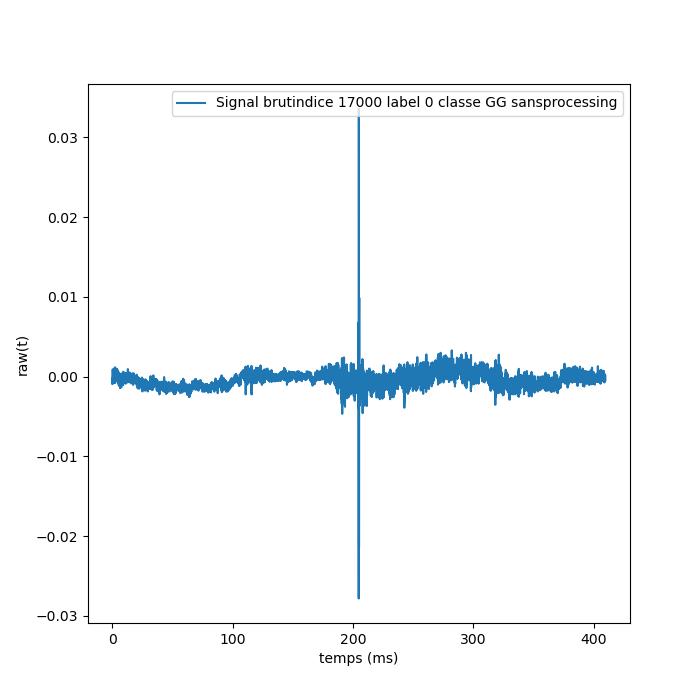
\includegraphics[width=\textwidth]{./images/indice17000Spectro1Dlabel0classeGGsansprocessingsanszoom.png}
  \end{subfigure}
  \begin{subfigure}[b]{0.3\textwidth}
    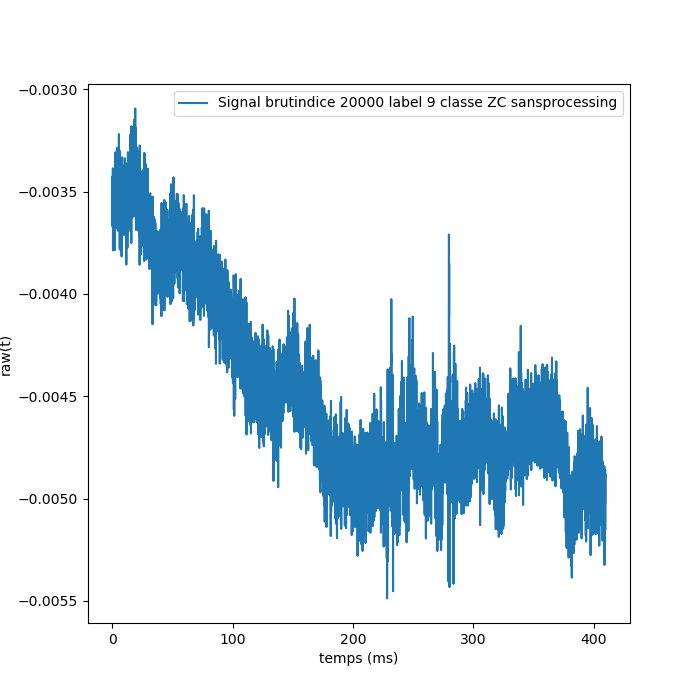
\includegraphics[width=\textwidth]{./images/indice20000Spectro1Dlabel9classeZCsansprocessingsanszoom.png}
    \caption{Signal 20000 brut}
  \end{subfigure}
  \begin{subfigure}[b]{0.3\textwidth}
    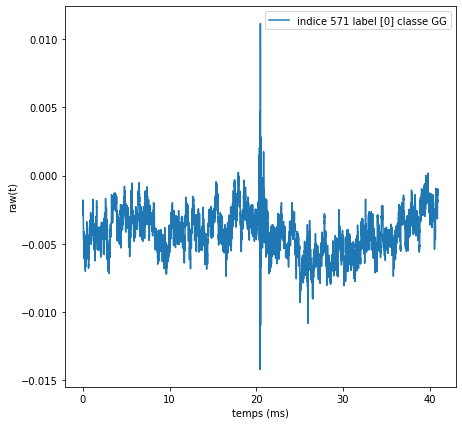
\includegraphics[width=\textwidth]{./images/indice571Spectro1Dlabel9classeZCsansprocessingsanszoom.png}
  \end{subfigure}
  \caption{Signaux 17000, 20000 et 571 bruts}
\end{figure}

On constate plusieurs choses tout d'abord il semble y avoir une certaine disparité entre les signaux certains étant beaucoup plus bruités que d'autres. De plus contrairement à ce que l'on pouvait penser le clic n'est pas toujours facile à distinguer et celui ci n'est pas non plus toujours bien centré.
Cependant on peut tirer quelques observations :
-Le clic semble durer 5 millisecondes
-L'amplitude des clics semble variable
-Il arrive que le bruit soit parfois suffisament important par rapport au clic pour rendre sont identification complexe voir impossible
Pour afiner notre analyse il parait pertinent de commencer par zoomer sur ce clic.
Pour cela il va donc faloir commencer par trouver un moyen d'isoler le clic.

\hypertarget{Le-zoom}{%}
\subsection{Le zoom}
\label{Le-zoom}}


\begin{figure}[!h]
  \centering
  \begin{subfigure}[b]{0.3\textwidth}
    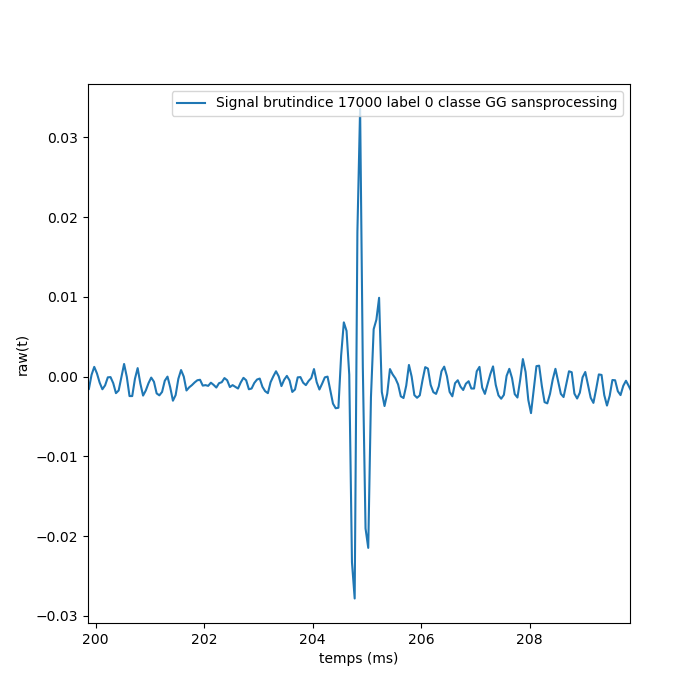
\includegraphics[width=\textwidth]{./images/indice17000Spectro1Dlabel0classeGGsansprocessingaveczoom.png}
  \end{subfigure}
  \begin{subfigure}[b]{0.3\textwidth}
    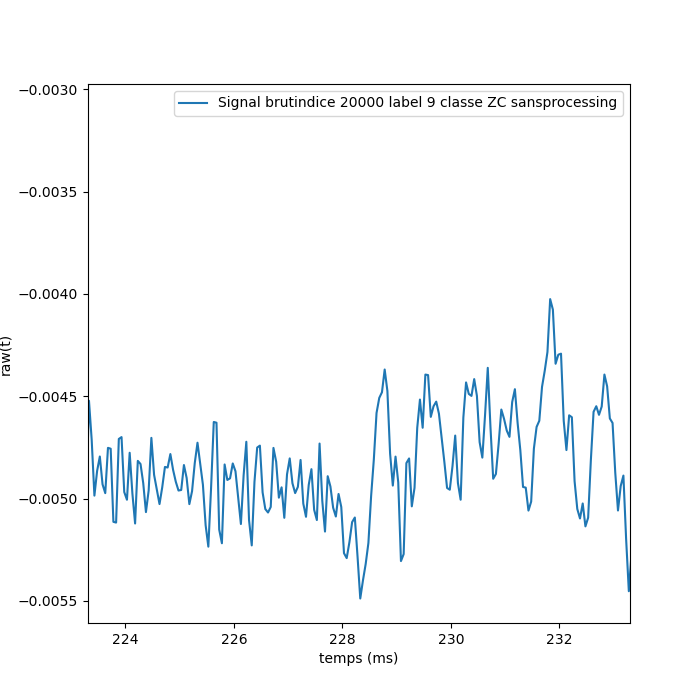
\includegraphics[width=\textwidth]{./images/indice20000Spectro1Dlabel9classeZCsansprocessingaveczoom.png}
  \caption{Signal 20000 zoom}
  \end{subfigure}
  \begin{subfigure}[b]{0.3\textwidth}
    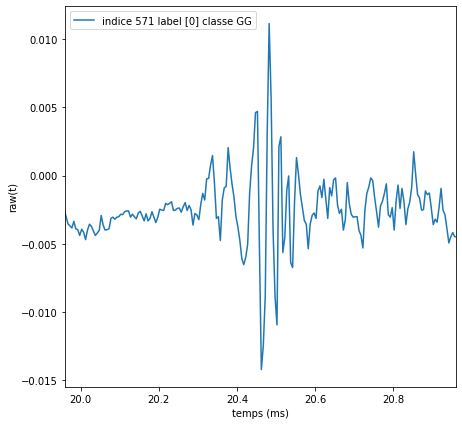
\includegraphics[width=\textwidth]{./images/indice571Spectro1Dlabel9classeZCsansprocessingaveczoom.png}
  \end{subfigure}
  \caption{Les signaux zoom}
\end{figure}

Pour zoomer sur le clic on commence par appliquer un filtre notament pour supprimer les bruits parasites(dont on parlera dans la partie traitement du signal) puis on identifie le maximum qui sera logiquement le milieu du clic puis on rajoute l'équivalent de la durée d'un clic avant et aprés ce maximum.

On constate plusieurs choses tout d'abord l'efficacité du zoom semble corélée à la qualité du signal de départ, de plus les "bons clics" semblent se situer aux alentours de 200 ms (ils sont donc bien centrés) même si leur intensité est très  variable pouvant aller jusqu'a un facteur 10 entre 2 clics. De plus sous cette forme nos observations semblent quand même limitées. On va donc commencer par les observer sous d'autres formes puis on cherchera à améliorer la qualité de nos signaux via diverses techniques. Etant donné la nature de nos données à savoir des enregistrements audios observer leurs spectrogrammes semble être le plus pertinent.

\hypertarget{Transformuxe9-de-Fourier}{%}
\subsection{Transformé de Fourier}
\label{Transformuxe9-de-Fourier}}
domaine temporel -> fréquenciel
Avant d'observer les spectrogrammes il convient de commencer par expliquer et observer les Transformés de Fourier de nos 3 signaux:
\begin{figure}[!h]
\centering
  \begin{subfigure}[b]{0.3\textwidth}
    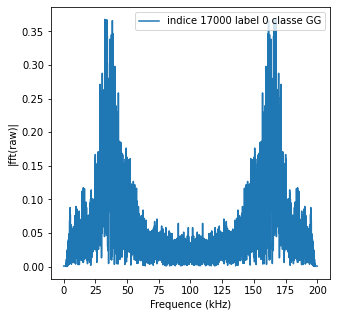
\includegraphics[width=\textwidth]{./images/17000fft.png}
  \end{subfigure}
  \begin{subfigure}[b]{0.3\textwidth}
    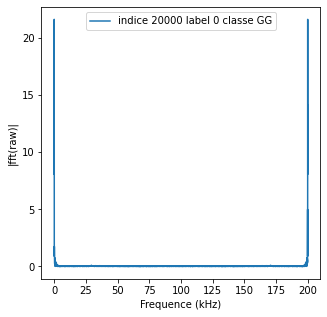
\includegraphics[width=\textwidth]{./images/20000fft.png}
  \end{subfigure}
  \begin{subfigure}[b]{0.3\textwidth}
    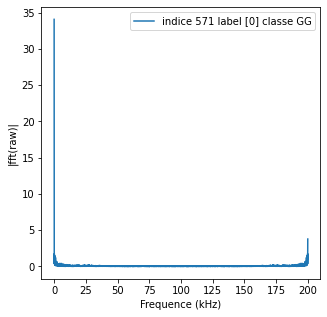
\includegraphics[width=\textwidth]{./images/571fft.png}
  \end{subfigure}
\caption{Transformé de Fourier des signaux 17000, 20000 et 571}
\end{figure}

\hypertarget{Spectrogrammes}{%}
\subsection{Spectrogrammes}
\label{Spectrogrammes}}

On commence tout d'abord par observer leurs Spectrogrammes en 2D:

\begin{figure}[!h]
  \centering
  \begin{subfigure}[b]{0.3\textwidth}
    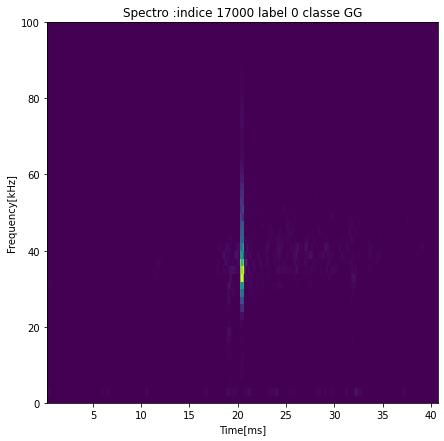
\includegraphics[width=\textwidth]{./images/indice17000Spectro2Dlabel0classeGGsansprocessingsanszoom.png}
  \end{subfigure}
  \begin{subfigure}[b]{0.3\textwidth}
    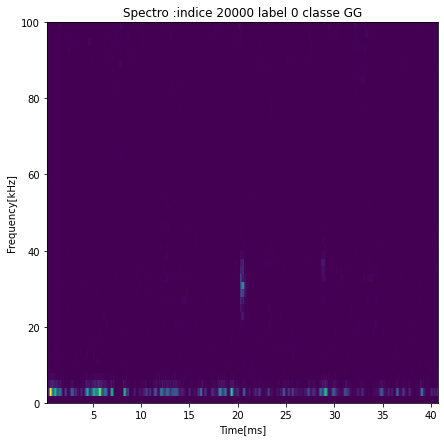
\includegraphics[width=\textwidth]{./images/indice20000Spectro2Dlabel9classeZCsansprocessingsanszoom.png}
  \end{subfigure}
  \begin{subfigure}[b]{0.3\textwidth}
    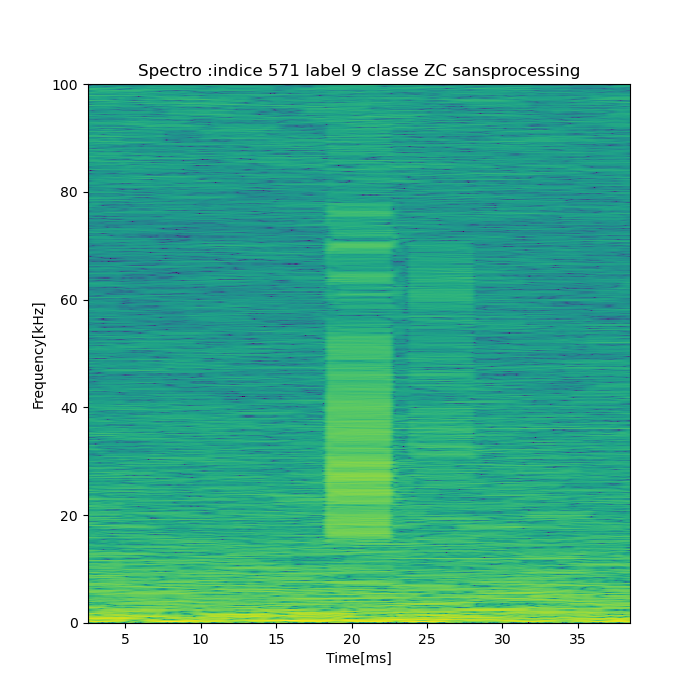
\includegraphics[width=\textwidth]{./images/indice571Spectro2Dlabel9classeZCsansprocessingsanszoom.png}
  \end{subfigure}
  \caption{Spectrogramme 2D des signaux}
\end{figure}

Puis les Spectrogrammes 3D:

\begin{figure}[!h]
\centering
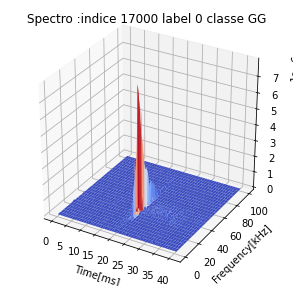
\includegraphics[width=4cm]{./images/indice17000Spectro3Dlabel0classeGGsansprocessingsanszoom.png}
\caption{Spectrogramme 3D du signal 17000}
\end{figure}
\begin{figure}[!h]
\centering
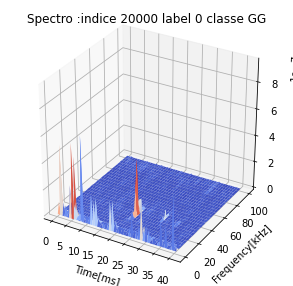
\includegraphics[width=4cm]{./images/indice20000Spectro3Dlabel9classeZCsansprocessingsanszoom.png}
\caption{Spectrogramme 3D du signal 20000}
\end{figure}

\begin{figure}[!h]
\centering
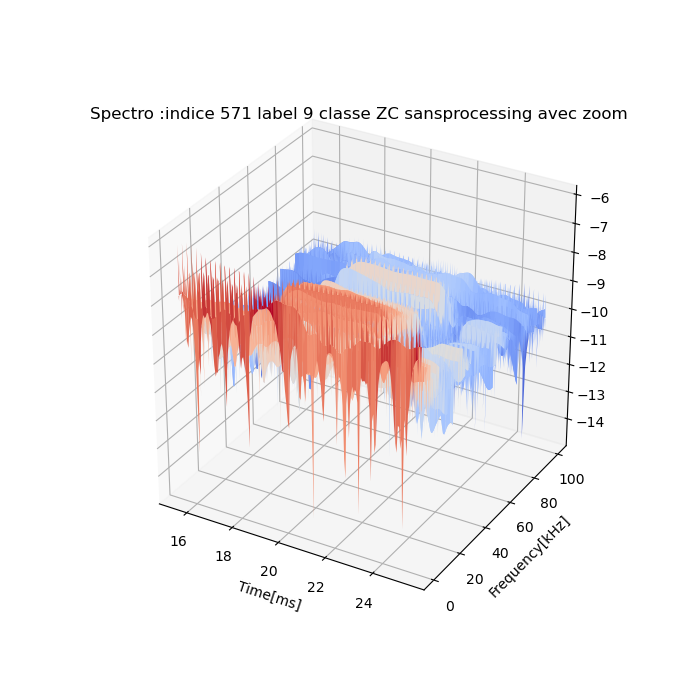
\includegraphics[width=4cm]{./images/indice571Spectro3Dlabel9classeZCsansprocessingaveczoom.png}
\caption{Spectrogramme 3D du signal 571}
\end{figure}

\hypertarget{Data-augmentation}
\subsection{Intérêt théorique}
\label{}}

Basiquement la Data augmentation regroupe un ensemble de méthodes permettant d'augmenter "artificiellement" la taille de la base sur laquelle notre ia va apprendre. Ainsi en plus de nos exemples initiaux on viendra rajouter de nouveaux exemples qui seront des versions "modifiées" des exemples initiaux.

Pour cela selon la nature des données de cette base on va par exemple :
-Rajouter du bruit sur les exemples
-Flouter les exemples s'il s'agit d'images
-Effectuer une rotation sur les exemples
-Modifier la luminosité dans le cas d'images
-Déplacer le clic dans le cas de notre probléme

L'intérêt le plus évident de cette opération est de simplement multiplier le nombre d'exemples disponibles afin d'éviter le surapprentissage mais elle peut avoir beaucoup plus d'utilité. En effet dans notre cas nous n'avons rencontré aucun probléme de surapprentissage mais nous avions besoin de l'utiliser pour une autre raison.
Effectivement nous avions remarqué que certains exemples avaient subis de fortes dégradations notament dues à du bruit ou bien à un fort décalage temporel du clic par exemple. Afin d'éviter que ces dégradations n'altérent le processus d'apprentissage de nos réseaux de neurones (le réseau pouvant par exemple assimiler une de ces dégradations a l'une des classes) plutôt que de supprimer ces dégradations il nous a paru plus pertinent de rajouter des exemples avec des dégradations similaires issuent d'exemples choisis aléatoirement parmis nos classes sur lesquelles ont aurait fait de la data augmentation. En effet ces dégradations pouvant être simplement dues a des problémes pendant l'enregistrement des clics (bateau navigant a proximité de l'animal ou encore d'autres animaux émettant divers bruits à proximité par exemple) il est plus que problable que les enregistrements qui seront soumis par la suite à notre classifieur contiennent également des dégradations qui ne devront pas entraver le bon fonctionnement de celui-ci.

\hypertarget{Rajout-de-bruit-blanc}
\subsection{Simulation de distance}
\label{Simulation-de-distance}}

\hypertarget{Traitement-du-signal}{%}
\section{Traitement du signal}
\label{Traitement-du-signal}}

Comme nous avons pu le voir précedement il arrive que certains enregistrements aient subis d'importantes dégradations, si dans un premier temps nous avons fait de la data augmentation il pouvait y avoir certains enregistrements pour lesquels cela ne suffis pas. Parcequ'ils seraient trop dégradés ils empêcheraient l'identification de l'espece, cela peut être un bruit tellement important qu'il recouvrirait le clic par exemple. Ainsi nous avons quand même dû faire du traitement du signal.

\hypertarget{Filtre-passe-haut}
\subsection{Mise à l'échelle}
\label{}}


\hypertarget{Les-Pipelines}{%}
\section{Les Pipelines}
\label{Les-Pipelines}}

A l'image des pipelines utilisés pour transporter le gaz ou le pétrole, les pipelines en informatique servent à transporter un flux de données.
Flux de données sur lequel on va effectuer un certain nombre d'opérations, flux qui sera ensuite injecté directement dans le réseau de neurones.
Cette méthode présente plusieurs interets majeurs :
-Premièrement elle nous évite de stocker le résultat des opérations intermédiaires  faisant gagner beaucoup de mémoire
-Deuxièmement elle nous permet d'optimiser grandement l'ensemble du processus de prétraitement des données.
-Troisièmement ce procédé améliore grandement les performances de tensorflow

En pratique l'ensemble de nos fonctions étaient stockées dans un fichier python nommé cachalot helper, et à chaque essai on faisait passer notre flux de données par les fonctions désirées avant de l'injecter dans le réseau de neurones.


\hypertarget{Les-PDF}{%}
\section{Les PDF (Fiches d'analyse)}
\label{Les-PDF}}

Les bases de données contenant un très grand nombre d'exemples (environs 90 000 au total que l'on peut visualiser sous 12 formes différentes soit potentiellement 1 080 000 images) afin de pouvoir exploiter les analyses faites précedement il a fallu créer un certain nombre d'outils afin de pouvoir aisement trier les données.
Pour cela je me suis inspiré du systéme de pipeline que nous venons de voir, ainsi dans un premier temps l'ensemble des fonctions nécessaires à l'analyse était stocké dans le cachalot_helper.

Dans un second temps j'ai créer dans un autre python une fonction paramètrable permettant tout d'abord de sélectionner ou un certain nombre de signaux dans un certain nombre de labels ou des signaux bien specifiques puis de générer (à l'aide du cachalot_helper) avec et ou sans preprocessing (les traitements du signal) avec ou sans zoom :
-Des plots des signaux sélectionnés
-Des spectrogrammes 2D des signaux sélectionnés
-Des spectrogrammes 3D des signaux sélectionnés
Une fois générés ils sont enregistrés sous forme de png dont le nom correspond à leur description ce qui donne par exemple pour le spectrogramme 3D sans processing et sans zoom de l'enregistrement numéro 17 000 de la classe GG dont le label est 0 :
indice17000Spectro3Dlabel0classeGGsansprocessingsanszoom.png. A noter que les plots simples sont enregistrés sous spectro1D pour des raisons pratiques.

Dans un troisième temps j'ai créer un autre python également paramètrable permettant de sélectionner des png en fonction de leur label de leur type (spectrogramme 1D ou 2D ou 3D) et leurs options (avec ou sans zoom et avec ou sans processing) puis ils sont stockés dans un ou plusieurs fichiers tex en fonction de leur nombre.

Dans un quatrième temps j'ai créer un autre python encore une fois paramètrable qui va récupérer les fichiers tex précedement créés puis les réunir dans un seul fichier tex qui va automatiquement s'executer pour générer un fichier pdf contenant l'ensemble des courbes qui étaient stockées dans les fichiers tex. Ce fichier pdf sera alors enregistré son nom correspondant à ce qu'il contient ainsi un fichier contenant les spectrogrammes 2D du label 6 sans processing et zoomer :sera nommer : Spectro2Dlabel6sansprocessingaveczoom.pdf

Et enfin un programme principal nommé apdfmaker également paramètrable chargé de faire tourner l'ensemble des programmes vus précedement afin de générer directement des fichiers pdf contenant ce que l'on désire. A noter que celui ci ne se contente pas de générer un pdf à la fois mais peut au contraire en générer une multitude à chaque run. Ainsi si l'on veut par exemple qu'il génére toutes les représentations graphiques possibles (soit 1 080 000 images) de tous les enregistrements puis qu'il les stock dans des pdf le plus détaillés possibles c'est parfaitement possible.

\hypertarget{conclusion}{%
\chapter{Conclusion}\label{conclusion}}

\section{Conclusion de l'étude}

Nous avons tout d'abord vu avec notre modèle de simulation qu'il fallait tout d'abord limité l'influence de l'aléatoire de notre simulations

\section{Piste d'amélioration}

\subsection{Changer architecture du réseau (Barabasi)}
Nous avons envisagé de changer la \textbf{topologie} \footnote{Topologie: Tel que la topologie d'un graffe il s'agit de la façon dont sont connecté nos neurones entre eux.}. Pour passer à une topologie dite \textbf{scalefree}. Qui est justement celle utilisé dans l'article d'origine. Cette architecture ressemble à ça:

\begin{figure}[h!]
\begin{center}
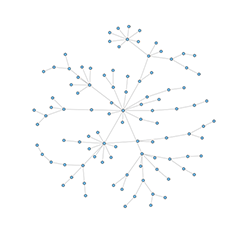
\includegraphics[width=10.5cm,height=10.5cm]{./images/scalefree.png}
\end{center}
\caption{Architecture scale-free}
\label{scale_free}
\end{figure}
\subsection{Réinterprétation de l'expérience}

Nous pouvons interpréter tout le réseau comme un utilisateur et cet entretient comme le temps qu'il accorde à la rumeur.

Cela permettrait
\section{Les apports du stage}
\subsection{les apports au monde}
Grâce à ce stage les chercheurs du laboratoire auront une idée plus précise de la diffusion d'un echo dans un réservoir et comment y créer un entretient ce qui sera utile pour leurs futures expériences. Cela permettra de mieux appréhender certains problèmes.
\subsection{les apports personels}
Comme dit pendant mon introduction, avant ce stage je n'avais aucune connaissance des réseaux de neurones, ce stage m'a donc permis de m'ouvrir a ce nouveau sujet passionnant, et m'a permis d'obtenir des compétence nécéssaire à mon cursus universitaire. Il m'a permis d'affiné mes méthodes de travail grâce à l'apprentissage de l'utilisation de GitHub et Colab. J'ai amélioré ma rédaction grace à l'approfondissement
du LaTeX. Il m'a permis d'affiner mon analyse de par l'analyse de mes résultats.


\cleardoublepage
\phantomsection
\bibliographystyle{plain} % Le style est mis entre accolades.
\addcontentsline{toc}{chapter}{Bibliographie}
\bibliography{biblioArekion}


\appendix
\include{biblioArekion}
%\include{bases}

\end{document}
